\subsection{Was ist Deployment}

Wenn man vom Deployment spricht, meint man die Bereitstellung von Software. Dies geschieht in der Regel durch halb- oder vollautomatisierte Prozesse, die die Installation und Konfiguration der Softwarelösungen durchführen. Im Deployment sind Aspekte wie die Installation, Konfiguration, Aktualisierung und Wartung von Systemen enthalten.
Die meisten IT-Organisationen und Softwareentwickler:innen führen regelmäßig Software-Updates und Patches mithilfe von teils vollautomatischen Prozessen durch. Es gibt verschiedene Arten von Deployment, die jeweils verschiedene Risiken mit sich bringen. Dennoch wird überall dasselbe Ziel verfolgt: Die Verteilung von Software auf Computern für Endbenutzer:innen.

\subsection{Verschiedene Arten von Deployment}

Grundsätzlich gibt es verschiedene Arten von Deployment. Diese werden prinzipiell folgendermaßen kategorisiert:
    \begin{itemize}
    \item Traditionelles Deployment
    \item Virtuelles Deployment
    \item Container Deployment
    \end{itemize}
\newpage
\subsection{Traditionelles Deployment}

Früher wurde eine Anwendung auf einem physischen Server deployed. Damals sah das ganze folgendermaßen aus.

Zunächst wurde ein physischer Server eingerichtet, auf dem ein Betriebssystem installiert wurde, das als Plattform für die auszuführende Software dient. Anschließend wurden auf diesem Server alle erforderlichen Tools oder Pakete, wie zum Beispiel Node oder NPM, installiert. Danach wurden sämtliche Dateien der Software auf den Server kopiert. Im letzten Schritt wird die Anwendung auf diesem Server gestartet, um sie funktionsfähig zu machen.


Solange nur eine einzige Anwendung auf diesem Server läuft, stellt dies kein Problem dar. Im Gegenteil, die Anwendung kann sehr performant auf dem Server laufen, da sie alle verfügbaren Ressourcen des Servers nutzen kann. Sobald jedoch mehrere Anwendungen auf einem Server laufen, können verschiedene Probleme auftreten, darunter:

\begin{itemize}
    \item Fehlende Ressourcen - auf einem physischen Server gibt es keine Möglichkeit, die Ressourcen für eine Applikation zu begrenzen. Eine Überlastung der Ressourcen kann somit den gesamten Server zum abstürzen bringen.
    \item Dateninkonsistenzen durch gemeinsam genutzten Speicher
    \item Es ist sehr teuer mehrere physische Server bereitzustellen.
\end{itemize}

\begin{figure}[h]
    \centering
    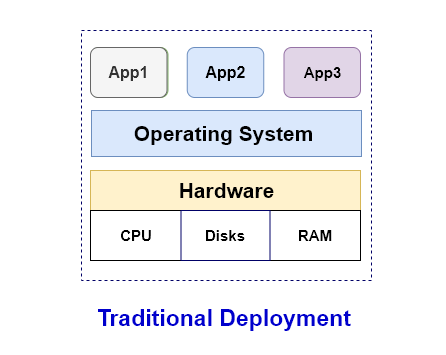
\includegraphics[width=0.7\linewidth]{pics/traditionelles-deployment.png}
    \caption{Traditionelles Deployment}
    \label{fig:enter-label}
\end{figure}


\cite{Traditional_vs_Container_vs_Virtuell_Deployment}

\newpage
\subsection{Virtuelles Deployment}
Um diese Probleme zu lösen, begann man die Software virtuell zu deployen. In diesem Fall wurde eine virtuelle Maschine erstellt, die über ihre eigene Partition im Speicher und ein eigenes Betriebssystem verfügte. Somit gab es keine Probleme mehr mit einer Ressourcenüberlastung und die individuellen Aplikationen konnten auch isoliert werden. Dennoch traten auch einige Probleme bei dieser Lösung auf, darunter:

\begin{itemize}
\item Betriebssysteme weisen eine beträchtliche Datenmenge auf und benötigen mehrere Gigabyte Speicherplatz.
\item Es dauert sehr lange die virtuelle Maschine zu starten.
\item  Die Anwendung ist nicht portabel
\end{itemize}

\begin{figure}[h!]
    \centering
    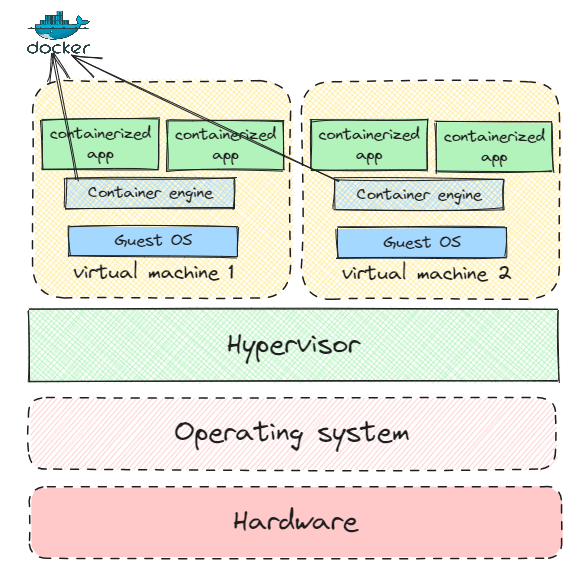
\includegraphics[width=0.7\linewidth]{pics/virtual-deployment.png}
    \caption{Virtual Deployment}
    \label{fig:enter-label}
\end{figure}

\cite{Virtuelles_Deployment}
\subsection{Container Deployment}
Um die Probleme des virtuellen Deployments zu überwinden, hat man sich entschieden, die Software nun in Containern zu deployen. Container sind eigenständige Einheiten, die den gesamten Anwendungscode sowie alle erforderlichen Abhängigkeiten in sich tragen. Neben Docker, einem der bekanntesten Tools zur Containerisierung von Anwendungen, stehen auch Alternativen wie Kubernetes und Podman zur Verfügung. Container bieten den Vorteil, dass sie sehr leichtgewichtig sind und daher innerhalb weniger Sekunden oder sogar Millisekunden gestartet werden können. Zudem sind Container im Gegensatz zu virtuellen Maschinen äußerst portabel und skalierbar.



\subsubsection{Vorgang des Container Deployment}

Als Erstes wird die gesamte Anwendung in ein Container Image verpackt. In diesem Image befindet sich der Anwendungscode, die Laufzeitumgebung und alle erforderlichen Abhängigkeiten wie zum Beipsiel Node oder NPM.

Als Nächstes wird das erstellte Container Image in einem Container-Image-Repository wie Docker Hub registriert und gespeichert.

Danach müssen die Container Images bereitgestellt werden, dies geschieht überlicherweise auf einem Container-Orchestrierungs-Framework wie Kubernetes, oder Docker Swarm.

Als letzten Schritt, muss der Container noch konfiguriert werden und mögliche Umgebungsvariablen werden gesetzt.

Wenn eine neue Version der Anwendung verfügbar ist, kann das Container-Deployment-Framework verwendet werden, um die Container schrittweise zu aktualisieren, ohne die Verfügbarkeit der Anwendung zu beeinträchtigen.


\begin{figure}[h!]
    \centering
    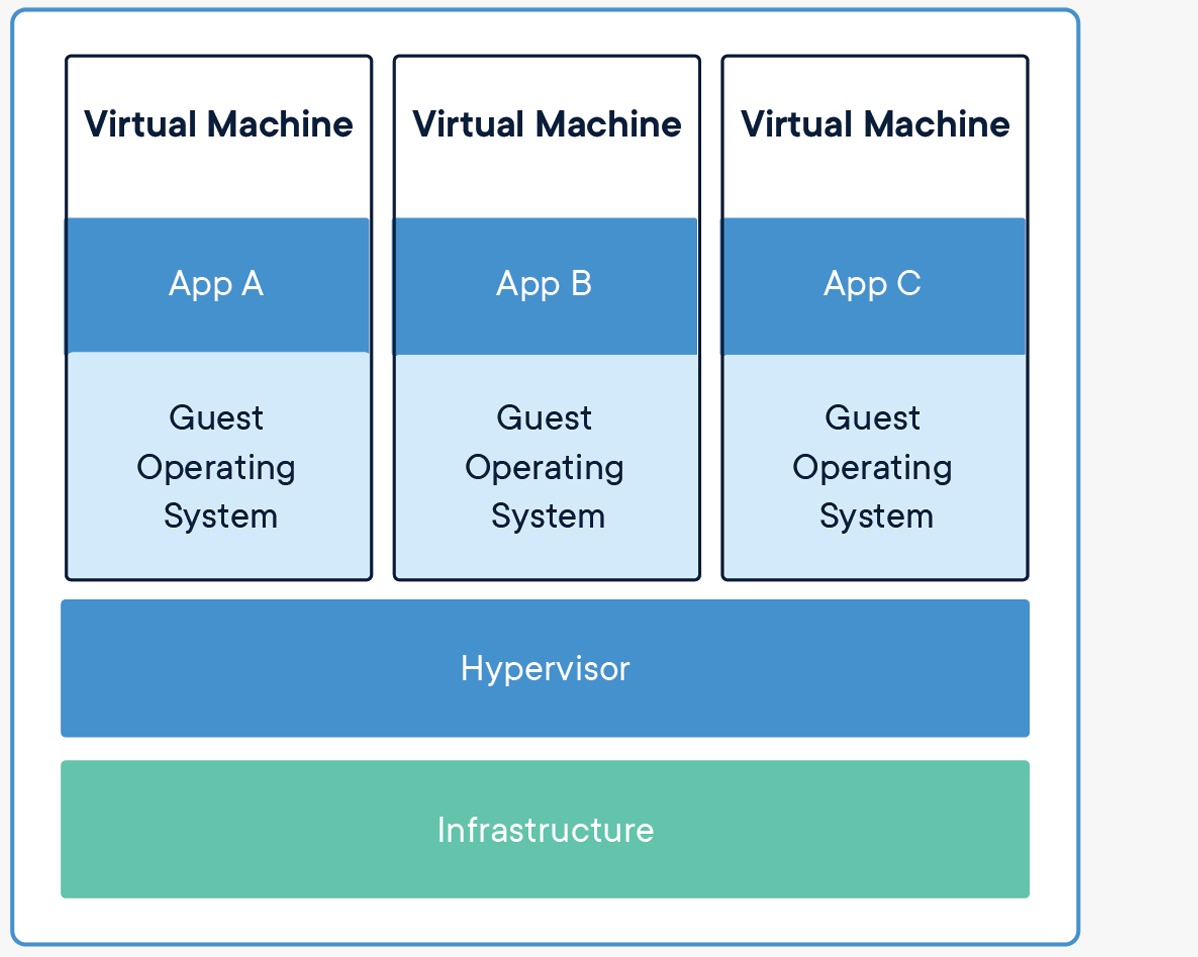
\includegraphics[width=0.6\linewidth]{pics/container_deployment.jpeg}
    \caption{Container Deployment}
    \label{fig:enter-label}
\end{figure}

\subsection{Umgebungsvariablen}

Umgebungsvariablen sind dazu da, um die Anwendungsgeheimnisse und Konfigurationen zu speichern, die wenn nötig von der Anwendung abgerufen werden können. Umgebungsvariablen verleihen einer Anwendung mehr Dynamik. Somit kann sehr schnell und einfach von internen auf externe Ressourcen geswitched werden. Der Wert einer Umgebungsvariable kann aus verschiedenen Quellen stammen, wie zum Beispiel Textdateien, Drittanbieter oder aufrufende Skripte. Das Wichtigste an den Umgebungsvariablen ist aber, dass der Wert nicht statisch gecoded ist sondern wirklich dynamisch und je nach Umgebung verändert werden kann.

Es gibt verschiedene Arten von Umgebungsvariablen:

\begin{itemize}
    \item \textbf{Systemumgebungsvariablen}
        \newline
        Diese Art von Umgebungsvariablen befinden sich im obersten Verzeichnis und laufen unter dem Benutzerprofil. In den meisten Fällen werden sie vom Systemadministrator festgelegt. Das wohl häufigste Vorkommen einer Systemumgebungsvariable ist die "PATH" Variable. Diese legt fest, in welchen Verzeichnissen gesucht wird, wenn ein Befehl in die Kommandozeile eingegeben wird.
        \cite{path_setzen}
        
    \item \textbf{Benutzer-Umgebungsvariablen}
        \newline
        In diesen Variablen wird zum Beispiel der Pfad zu einer lokal installierten Bibliothek gespeichert, welche nur von manchen Benutzern:innen verwendet werden. Für Änderungen an dieser Variable werden die Systemadministrator:innen nicht benötigt. Diese Variablen sind sehr hilfreich, um lokale Änderungen nur für einen Benutzer gültig zu machen.
    \item \textbf{Laufzeit-/Prozessumgebungsvariablen}
        \newline
        Auf diese Art von Umgebungsvariablen haben die Benutzer:innen mehr oder weniger keinen Einfluss. Die Lebensdauer dieser Umgebungsvariablen ist durch den übergeordneten Prozess begrenzt, der sie erstellt hat.
        Sollte es aber den speziellen Fall geben, dass die Benutzer:innen Einfluss auf die Laufzeitumgebungsvariablen braucht, dann kann er diese im Terminal-Skript erstellen.
\end{itemize}

Im Falle diese Diplomarbeit wurden Umgebungsvariablen hauptsächlich verwendet um die Sicherheit aufrecht zu erhalten und datenbankbezogene Informationen oder API - Keys darin zu speichern.

\subsubsection{.env-Dateien}
In dieser Diplomarbeit wurden .env Files verwendet um die Umgebungsvariablen zu speichern. Die Anwendung ist sehr simpel. Es muss im Stammverzeichnis des Projektes eine .env Datei angelegt werden, in dieser können nach folgendem Schema die Umgebungsvariablen definiert werden:
\begin{verbatim}
    VAR_UNO=SOME_KEY_HERE
    VAR_DOS=SOME_OTHER_KEY_HERE
\end{verbatim}

Wenn diese Variablen von der Anwendung benötigt werden, sucht diese danach und lädt sie während der Laufzeit ins Programm. 
Es können allerdings auch mehrere Dateien, für mehrere Umgebungen erstellt werden z.B
\begin{verbatim}
    .env.dev -> Fuer die Developement Umgebung
    .env.prod -> Fuer die Production Umgebung
\end{verbatim}

Wichtig ist außerdem noch, die .env Dateien nicht in eine Versionskontrolle wie Github aufzunehmen. Wenn ein spezielles Schema definiert wurde, welches auch für andere Entwickler wichtig ist, erstellt man in den meisten Fällen eine .env.template Datei und definiert hier das Schema folgendermaßen:

\begin{verbatim}
    VAR_UNO= # Your value here
    VAR_DOS= # Your value here
\end{verbatim}

Somit ist das Schema bekannt, aber vertrauliche Werte werden nicht in die Versionskontrolle mit aufgenommen.


\cite{Umgebungsvariablen}




\subsection{Docker}

Docker wurde erstmals im März 2013 von dotCloud veröffentlicht und nutzt den Linux-Kernel und seine Ressourcenkontrollmechanismen wie Cgroups und Namespaces, um Prozesse zu isolieren, wodurch sie in voneinander unabhängigen Umgebungen ausgeführt werden können. Dieser fundamentale Aspekt der Container-Technologie, ermöglicht die parallele Ausführung mehrerer Prozesse und Anwendungen in isolierten Containern. Dies steigert die Effizienz Ihrer Infrastruktur, ohne dabei die Sicherheitsvorteile zu vernachlässigen, die sich aus der Nutzung separater Umgebungen ergeben.

Container-Tools, wie zum Beispiel Docker, arbeiten mit einem imagebasierten Deployment-Modell. Dies erleichtert die Anwendung und Nutzung von gemeinsamen Ressourcen und Services mit sämtlichen Abhängigkeiten.

Mit Docker ist es möglich einen Teil einer Anwendung zu aktualisieren oder zu reparieren ohne die gesamte Anwendung deaktivieren zu müssen. Außerdem besitzt Docker ein Rollbacking, also das zurücksetzen auf die vorherige Version.

\begin{figure}[h!]
    \centering
    
\includegraphics[width=0.7\linewidth]{pics/docker-logo.png}
    \caption{Docker Logo}
    \label{fig:enter-label}
\end{figure}

\subsubsection{Container}
Ein Container ist eine standardisierte Einheit von Software, die den Code sowie alle benötigten Abhängigkeiten zusammenfasst. Dadurch kann die Anwendung schnell und zuverlässig von einer Rechenumgebung in eine andere verschoben werden. Ein Docker-Containerimage ist ein schlankes, eigenständiges und ausführbares Softwarepaket. Es beinhaltet alles Notwendige, um eine Anwendung auszuführen: den Code selbst, die Laufzeitumgebung, Systemwerkzeuge, Systembibliotheken und Einstellungen.\newline

Während der Ausführung werden Containerimages zu Containern. Im Fall von Docker-Containern geschieht dies, wenn sie auf der Docker Engine laufen. Diese Technologie ist sowohl für Linux- als auch für Windows-Anwendungen verfügbar. Containerisierte Software wird unabhängig von der zugrunde liegenden Infrastruktur immer konsistent arbeiten. Container isolieren die Software von ihrer Umgebung und gewährleisten eine gleichbleibende Funktionalität, selbst wenn sich die Umgebungen, beispielsweise zwischen Entwicklungs- und Produktionsumgebungen, unterscheiden.

\begin{figure}[h!]
    \centering
    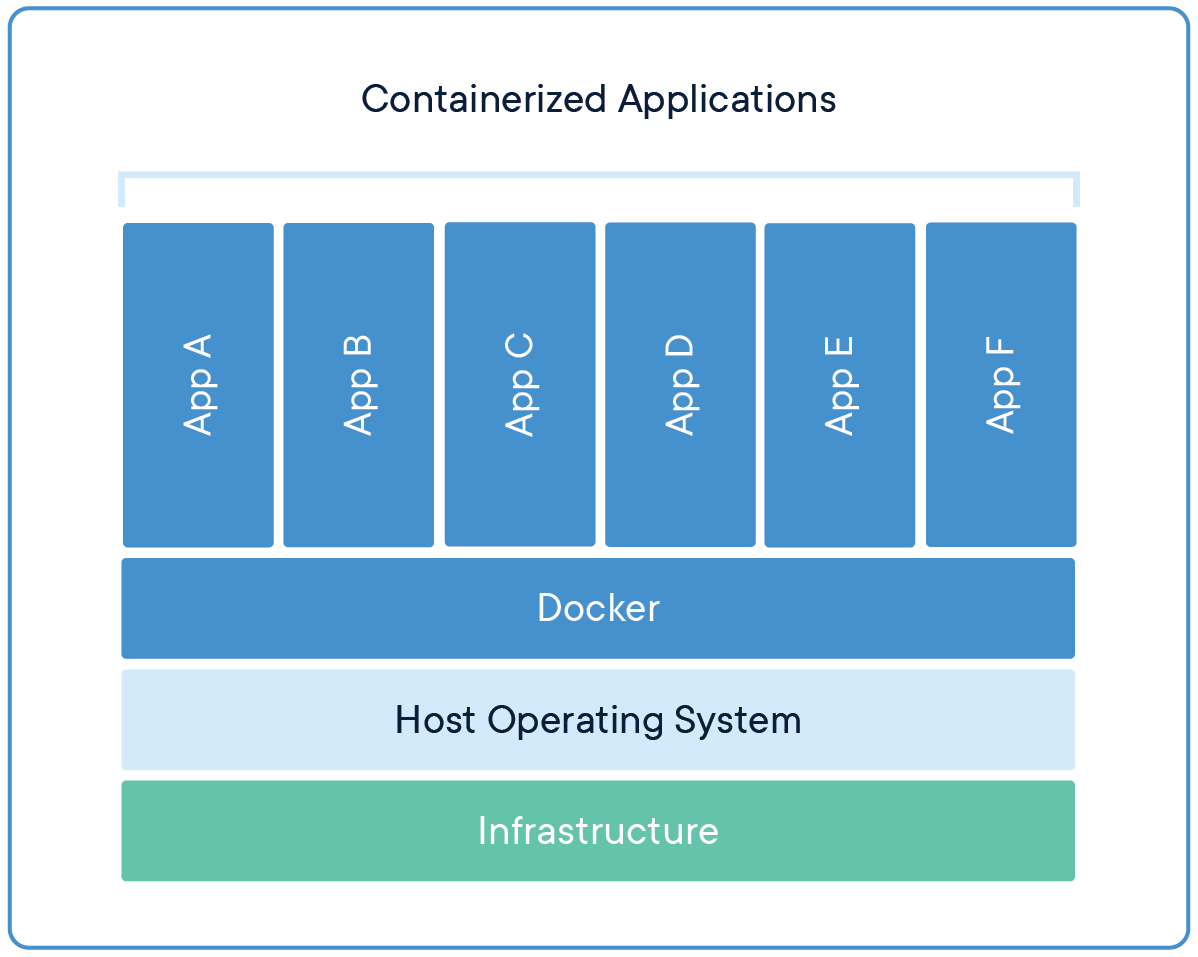
\includegraphics[width=0.7\linewidth]{pics/docker-container.png}
    \caption{Container Deployment}
    \label{fig:enter-label}
\end{figure}

\cite{Vorteile_Nachteile_Docker}
\cite{Was_ist_Docker}




